\documentclass[]{article}
\usepackage{graphicx}
\usepackage{amsmath}
\usepackage{framed}
%opening
\title{RgoogleMaps}

\begin{document}

%\maketitle

\section{RgoogleMaps}

\begin{framed}
\begin{verbatim}
library(RgoogleMaps)

lat <- c(48,64) #define our map's ylim
lon <- c(-140,-110) #define our map's xlim
center <- c(mean(lat), mean(lon))  
zoom <- 5  

#zoom: 1 = furthest out (entire globe)   
#      larger numbers = closer in

terrmap <- GetMap(center=center, zoom=zoom, 
    maptype= "terrain", 
    destfile = "terrain.png") 
\end{verbatim}
\end{framed}
\begin{figure}[h!]
\centering
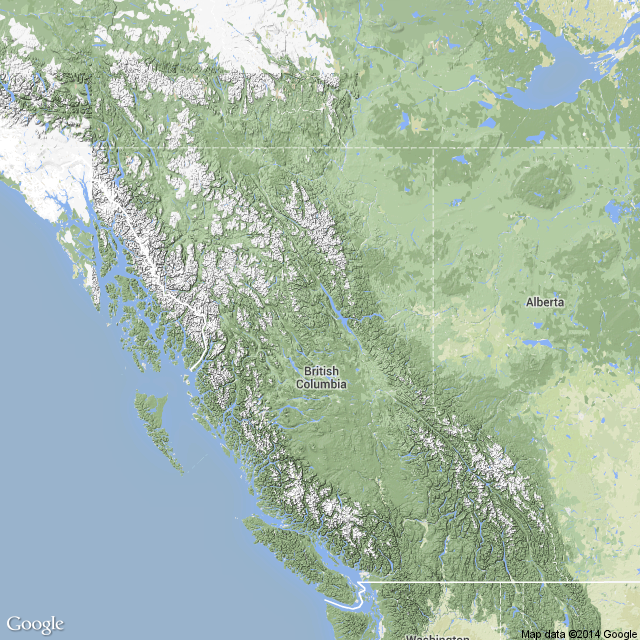
\includegraphics[width=0.9\linewidth]{./terrain}
%\caption{}
\label{fig:terrain}
\end{figure}
%#lots of visual options, just like google maps: 
%# maptype = c("roadmap", "mobile", "satellite", "terrain", 
%# "hybrid", "mapmaker-roadmap", "mapmaker-hybrid")
\end{document}